\documentclass[12pt]{article}

\usepackage[]{graphicx}
\usepackage[]{color}
\usepackage{alltt}

\newcommand{\mytitle}{Uncertainty Quantification in Neural Networks}
\newcommand{\myname}{Baisu Zhou}
\newcommand{\mysupervisor}{Dr.\@ Ludwig Bothmann}

\usepackage[a4paper, width = 160mm, top = 35mm, bottom = 30mm, 
bindingoffset = 0mm]{geometry}
\usepackage[utf8]{inputenc}
\usepackage{ragged2e}
\usepackage{xcolor}
\usepackage[round, comma]{natbib}
\usepackage{fancyhdr}
\newcommand{\changefont}{%
    \fontsize{8}{11}\selectfont
}
\usepackage{hyperref}
\hypersetup{
  colorlinks = true,
  linkcolor = black,
  urlcolor = black,
  citecolor = black}

\pagestyle{fancy}
\fancyhead{}
\fancyhead[R]{\changefont{\mytitle}}
\fancyfoot{}
\fancyfoot[R]{\thepage}
\setlength{\headheight}{14.5pt}
\setlength{\parindent}{1em}
\interfootnotelinepenalty = 10000

\usepackage{amsmath, amssymb}
\usepackage{bm}
\usepackage{mathtools}
\usepackage{derivative}
\usepackage{fixdif}
\usepackage{mleftright}

\newcommand{\simiid}{\overset{iid}{\sim}}

\newcommand{\RR}{\mathbb{R}}
\newcommand{\XX}{\mathbb{X}}
\newcommand{\YY}{\mathbb{Y}}

\renewcommand{\vec}[1]{\bm{#1}}
\newcommand{\mat}[1]{\bm{\mathbf{#1}}}

\newcommand{\T}{\top}
\newcommand{\wc}{\,\cdot\,}
\newcommand{\defeq}{\coloneqq}
\newcommand{\given}{\,|\,}
\newcommand{\Given}{\,\middle|\,}

\newcommand{\set}[1]{\left\{#1\right\}}
\newcommand{\abs}[1]{\left\vert #1 \right\vert}
\newcommand{\norm}[1]{\left\| #1 \right\|}

\newcommand{\grad}{\nabla}

\DeclareMathOperator{\Ind}{\mathbb{I}}
\DeclareMathOperator{\Exp}{\mathbb{E}}
\DeclareMathOperator{\Var}{\mathbb{V}}
\DeclareMathOperator*{\argmin}{\arg\min}
\DeclareMathOperator*{\argmax}{\arg\max}

\newcommand{\emprisk}{R_{\textup{emp}}}
\newcommand{\regrisk}{R_{\textup{reg}}}
\newcommand{\loss}{\mathcal{L}}
\usepackage[capitalise]{cleveref}
% ------------------------------------------------------------------------------
% MAIN -------------------------------------------------------------------------
% ------------------------------------------------------------------------------
\IfFileExists{upquote.sty}{\usepackage{upquote}}{}
\begin{document}

% FRONT PAGE -------------------------------------------------------------------
 
\begin{titlepage}
\begin{center}
    
\LARGE
Seminar Paper
    
\vspace{0.5cm}
      
\rule{\textwidth}{1.5pt}
\LARGE
\textbf{\mytitle}
\rule{\textwidth}{1.5pt}
   
\vspace{0.5cm}
      
\large
Department of Statistics \\
Ludwig-Maximilians-Universität München 

\vfill

\Large
\textbf{\myname}

\vfill

\large
Munich, Feburary 28\textsuperscript{th}, 2025
      
\vfill


\includegraphics[width = 0.4\textwidth]{sigillum.png}

\vfill

\normalsize
Submitted in partial fulfillment of the requirements for the degree of B. Sc.
\\

Supervised by \mysupervisor

\end{center}
\end{titlepage}

% CONTENTS ---------------------------------------------------------------------

\pagenumbering{Roman}
\newpage

\begin{abstract}

Quantifying uncertainty in predictions is a way to make neural networks as highly complex black-box models more trustworthy. Following a Bayesian approach, one can turn neural networks into probabilistic models capable of estimating uncertainty along with making predictions. However, tracking uncertainty in neural networks imposes great computational challenges. In this paper, we present the theoretical framework and discuss approaches that make uncertainty-aware deep learning feasible.

\end{abstract}

\newpage
\tableofcontents

%%%% if you would want to include material overview
%%%% use one of the following in addition
% \newpage
% \listoffigures
% \newpage
% \listoftables
\newpage

% CHAPTERS ---------------------------------------------------------------------

\pagenumbering{arabic}

\section{Introduction}
\label{sec:intro}

Deep neural netwrks (DNNs) have demonstrated astonishing capabilites of tackling complex predictive tasks in computer vision, natural language processing, and various other fields of science and engineering. While they are often able to achieve high predictive accuracy given large volumes of training data, DNNs are often untrustworthy in real-world applications.

Recent research has highlighted that noisy, corrupted input data can easily mislead neural networks to make wrong predictions. For instance, covering a part of the input image with noise causes a DNN-based vehicle control system to fail at steering angle prediction, which could put human lives in danger \citep{loquercioAutoDrive2020}. Even a barely perceptible noise, if designed in a certain way, can completely irritate DNN image classifiers \citep{moosaviAdversarial2017}. In the other extreme, certain noise patterns unrecognizable to humans get classified by neural networks as wild animals or everyday objects, and the predictive probabilities assigned to these false classes are very high \citep{nguyenFoolingDNN2015}. Predictions with unreasonably high confidence are not limited to the case where the input data are fine-tuned noise. \cite{guoCalibration2017} showed that over-confidence is a common phenomenon in DNNs. Apart from the objective shortcomings, how human users perceive neural networks also plays a role. In the clinical context, for example, people tend not to trust neural networks due to their nature of being black-box models \citep{royBrainSegment2019}.

One approach to making neural networks more trustworthy is to equip them with uncertainty estimation. Besides the predicted label, the model should report the degree of uncertainty in its prediction. If the potentialy unreliable model is uncertain, a reliable human expert can be called to intervene.

In \cref{sec:bayesian-dl}, we present the Bayesian framework for uncertainty quantification in neural networks. After setting up this theoretical foundation, we introduce three popular uncertainty quantification methods. In \cref{sec:la}, we derive Laplace approximation and present some of its extensions. In \cref{sec:de}, we motivate the use of ensemble methods for uncertainty quantification from a Bayesian perspective. In \cref{sec:mcd}, we introduce Monte Carlo Dropout, which can be motivated as an ensemble method but enjoys a Bayesian justification. Finally, we apply these methods on toy experiments in \cref{sec:exp}.

\newpage
\section{Bayesian Deep Learning}
\label{sec:bayesian-dl}

Adopting a Bayesian view, we use probability distributions to capture uncertainty. This section delves into setting up the framework of Bayesian inference in the context of deep learning.  

\subsection{Neural Networks as Probabilistic Models}
\label{sec:nn}

A neural network is a parametric function $f(\wc; \vec{\theta})$ mapping feature objects $x \in \mathcal{X}$ to target values or labels $f(x; \vec{\theta}) \in \mathcal{Y}$, where $\vec{\theta}$ is a typically high-dimensional parameter vector. In preparation for a Bayesian interpretation, we view neural network from a probabilistic modeling perspective and establish the equivalence between empirical risk minimization and maximum likelihood estimation.

Let $\mathcal{D} = \{(\vec{x}_i, y_i)\}_{i=1}^{n}$ be a training set. We assume the training observations to be i.i.d. For a regression task, in which the network is intended to predict scalar labels, we make the distributional assumption
\begin{equation*}
  y_i \given \vec{x}_i \overset{iid}{\sim} \mathcal{N}(f(\vec{x}_i; \vec{\theta}); \sigma^2).
\end{equation*}
The negative log-likelihood on $\mathcal{D}$ is given by
\begin{equation*}
  - \log p(\mathcal{D} \given \vec{\theta}) = \sum_{i=1}^{n} - \log p(y_i \given \vec{x}_i, \vec{\theta})
  \propto \sum_{i=1}^{n} (y_i - f(\vec{x}_i; \vec{\theta}))^2,
\end{equation*}
which can be interpreted an empirical risk w.r.t.\@ the square loss. In this approach, the variance parameter $\sigma^2$ is assumed to be a constant and ignored in the optimization procedure, although the conditional variance can be seen as a natural measure of uncertainty for the target variable. To use this measure, we can predict $\sigma^2$ from training data. Accounting for potential heteroskedasticity, we use a network with two outputs: one for the predicted mean $\mu_i \defeq \mu(\vec{x}_i; \vec{\theta})$, the other for the predicted variance $\sigma^2_i \defeq \sigma^2(\vec{x}_i; \vec{\theta})$. The distributional assumption becomes
\begin{equation*}
  y_i \given \vec{x}_i \overset{iid}{\sim} \mathcal{N}(\mu(\vec{x}_i; \vec{\theta}); \sigma^2(\vec{x}_i; \vec{\theta})).
\end{equation*}
The corresponding negative log-likelihood is a sum of logarithms of Gaussian densities.

For a binary classification task, the network outputs a predictive probability for the positive class. The only appropriate distributional assumption is a Bernoulli distribution
\begin{equation*}
  y_i \given \vec{x}_i \overset{iid}{\sim} \operatorname{Ber}(f(\vec{x}_i; \vec{\theta})).
\end{equation*}
Then the negative log-likelihood on $\mathcal{D}$ amounts to an empirical risk w.r.t.\@ the Bernoulli loss
\begin{equation*}
  - \log p(\mathcal{D} \given \vec{\theta})
  = \sum_{i=1}^{n} - y_i \log f(\vec{x}_i; \vec{\theta}) - (1 - y_i) \log (1 - f(\vec{x}_i; \vec{\theta})).
\end{equation*}
For a multiclass classification task, the network outputs a probability vector of $K$ entries. Each entry represents the predictive probability for one of the $K$ classes. We consider each label $y_i$ to be a class index, i.e., $y_i \in \{1, \dots, K\}$, and assume the conditional distribution of $y_i$ given $\vec{x}_i$ to be a categorical distribution
\begin{equation*}
  y_i \given \vec{x}_i \overset{iid}{\sim} \operatorname{Cat}(f(\vec{x}_i; \vec{\theta})),
\end{equation*}
which yields
\begin{equation*}
  - \log p(\mathcal{D} \given \vec{\theta})
  = \sum_{i=1}^{n} \sum_{k=1}^{K} - \Ind(y_i = k) \log f(\vec{x}_i; \vec{\theta}),
\end{equation*}
where $\Ind(\wc)$ denotes the indicator function. This negative log-likelihood corresponds to an empirical risk w.r.t.\@ the cross entropy loss.

Defining the empirical risk as
\begin{equation*}
  \emprisk(\vec{\theta}) \coloneqq - \log p(\mathcal{D} \given \vec{\theta}) = \sum_{i=1}^{n} \loss(y_i, f(\vec{x}_i; \vec{\theta})),
\end{equation*}
where $\loss$ is a loss function derived from the negative log-likelihood, we see that the empirical risk minimizer
\begin{equation*}
  \hat{\vec{\theta}} \coloneqq \argmin_{\vec{\theta}} \emprisk(\vec{\theta}) = \argmax_{\vec{\theta}} \log p(\mathcal{D} \given \vec{\theta})
\end{equation*}
is identical to the maximum likelihood estimator of $\vec{\theta}$. In practice, \emph{gradient descent} is used to solve the minimization problem. The algorithm starts at a random initial point $\vec{\theta}^{(0)}$ in the parameter space and iteratively computes
\begin{equation*}
  \vec{\theta}^{(t+1)} \coloneqq \vec{\theta}^{(t)} - \eta \grad \emprisk\left( \vec{\theta}^{(t)} \right) = \vec{\theta}^{(t)} - \eta \grad \sum_{i=1}^{n} \loss(y_i, f(\vec{x}_i; \vec{\theta}))
\end{equation*}
for $t = 1,2,\dots$ until convergence. The hyperparameter $\eta > 0$ is called the learning rate, which may also depend on $t$. If the training set is large, it is too expensive to re-evaluate the gradient $\grad \emprisk(\vec{\theta}^{(t)})$ in every iteration $t$. For computational efficiency, we randomly sample a \emph{mini-batch} $\mathcal{B} \subseteq \mathcal{D}$ of training data and estimate the gradient by
\begin{equation*}
  \frac{n}{\abs{\mathcal{B}}} \sum_{(\vec{x}, y) \in \mathcal{B}} \ell(\vec{x}, y).
\end{equation*}
In every iteration, we generate a new random mini-batch, estimate the loss gradient, and use this estimate to perform gradient descent. This training procedure is called \emph{stochastic gradient descent (SGD)}.

\subsection{Regularization and MAP Estimation}
\label{sec:regularization}

As highly complex functions, neural networks are prone to overfitting. For higher generalizability, regularization is necessary. L2 regularization is commonly used in deep learning. Instead of the empirical risk, we now minimize the \emph{regularized risk}
\begin{equation*}
  \regrisk(\vec{\theta}) \coloneqq \emprisk(\vec{\theta}) + \frac{\lambda}{2} \norm{\vec{\theta}}^2,
\end{equation*}
where $\norm{\wc}$ denotes the Euclidean norm and $\lambda > 0$ is a hyperparameter parameter controling the strength of regularization\footnote{Scaling $\lambda$ by $1/2$ simplifies the gradient.}. In practice, L2 regularization is implemented efficiently as \emph{weight decay}. Note that
\begin{align*}
  \grad \regrisk(\vec{\theta}) = \grad \emprisk(\vec{\theta}) + \lambda \vec{\theta}.
\end{align*}
When performing gradient descent under L2 regularization, the update rule becomes
\begin{align*}
  \vec{\theta}^{(t+1)} &= \vec{\theta}^{(t)} - \eta \grad \regrisk\left( \vec{\theta}^{(t)} \right) \\
  &= \vec{\theta}^{(t)} - \eta \left( \grad \emprisk\left( \vec{\theta}^{(t)} \right) + \lambda \vec{\theta}^{(t)} \right) \\
  &= \vec{\theta}^{(t)} - \eta \grad \emprisk(\vec{\theta}) - \eta \lambda \vec{\theta}^{(t)} \\
  &= (1 - \eta \lambda) \vec{\theta}^{(t)} - \eta \grad \emprisk\left( \vec{\theta}^{(t)} \right).
\end{align*}
Given that $\eta \lambda < 1$, the parameters first decay by a factor $(1 - \eta \lambda)$ before the usual gradient step, hence the name ``weight decay.''

Now we show the equivalence between L2 regularization or weight decay and Bayesian \emph{maximum a posteriori (MAP)} estimation with a Gaussian prior $\vec{\theta} \sim \mathcal{N}(0, \tau^2 I)$. Suppose $\emprisk(\vec{\theta}) = - \log p(\mathcal{D} \given \vec{\theta})$. The parameter estimate under L2 regularization is given by
\begin{equation} \label{eq:l2-reg}
  \hat{\vec{\theta}}_\text{L2} \coloneqq \argmin_{\vec{\theta}} \left( \emprisk(\vec{\theta}) + \frac{\lambda}{2} \norm{\vec{\theta}}^2 \right)
  = \argmin_{\vec{\theta}} \left( - \log p(\mathcal{D} \given 
  \vec{\theta}) + \frac{\lambda}{2} \norm{\vec{\theta}}^2 \right).
\end{equation}
Under the prior assumption $\vec{\theta} \sim \mathcal{N}(0, \tau^2 I)$, the MAP estimate or \emph{posterior mode} is given by
\begin{align*}
  \hat{\vec{\theta}}_\text{MAP} &\coloneqq \argmax_{\vec{\theta}} \log p(\vec{\theta} \given \mathcal{D}) \\
  &= \argmax_{\vec{\theta}} \left( \log p(\mathcal{D} \given \vec{\theta}) + \log p(\vec{\theta}) \right) \\
  &= \argmax_{\vec{\theta}} \left( \log p(\mathcal{D} \given \vec{\theta}) - \frac{1}{2 \tau^2} \norm{\vec{\theta}}^2 \right) \\
  &= \argmin_{\vec{\theta}} \left( - \log p(\mathcal{D} \given \vec{\theta}) + \frac{1}{2 \tau^2} \norm{\vec{\theta}}^2 \right).
\end{align*}
Setting $\tau^2 = \lambda^{-1}$ gives exactly \eqref{eq:l2-reg}. Therefore, if a network is trained using weight decay, we can interpret the parameter estimate as an MAP estimate.

\subsection{Predictive Distribution}
\label{sec:bma}

Given a single MAP estimate $\hat{\vec{\vec{\theta}}}$ and a new feature vector $\vec{x}_*$, one could directly use the likelihood $p(y_* \given \vec{x}_*, \hat{\vec{\vec{\theta}}})$ to express uncertainty about the predicted target $y_*$. From a Bayesian perspective, however, we know that the MAP estimate is merely a single point from the posterior. A more reliable representation of the predictive uncertainty should take all information from the posterior into account. This motivates the \emph{predictive distribution}
\begin{equation} \label{eq:predictive}
  p(y_* \given \vec{x}_*, \mathcal{D}) \defeq \int p(y_* \given \vec{x}_*, \vec{\vec{\theta}}) p(\vec{\vec{\theta}} \given \mathcal{D}) \d\vec{\vec{\theta}}
  = \mathbb{E}_{\vec{\vec{\theta}} \sim p(\vec{\vec{\theta}} \given \mathcal{D})}[p(y_* \given \vec{x}_*, \vec{\vec{\theta}})].
\end{equation}
The integral is also called \emph{Bayesian model averaging} \citep{wilsonBayesianDeepLearning2020}. Instead of focusing on a single point estimate, the predictive distribution averages over the entire posterior. Since the posterior distribution is tractable, the true predictive distribution is generally unknown. Even if an approximation of the posterior exists, the integral in \eqref{eq:predictive} is typically intractable \citep{wilsonBayesianDeepLearning2020,gawlikowskiSurveyUQ2023}. A generic approach to approximating this integral is \emph{Monte Carlo integration}. The idea is to approximate the expectation by a sample mean
\begin{equation*}
  p(y_* \given \vec{x}_*, \mathcal{D})
  = \mathbb{E}_{\vec{\vec{\theta}} \sim p(\vec{\vec{\theta}} \given \mathcal{D})}[p(y_* \given \vec{x}_*, \vec{\vec{\theta}})]
  \approx \frac{1}{m} \sum_{i=1}^{m} p(y_* \given \vec{x}_*, \hat{\vec{\vec{\theta}}}_i),
\end{equation*}
where $\hat{\vec{\vec{\theta}}}_1, \dots, \hat{\vec{\vec{\theta}}}_m$ are an i.i.d.\@ sample drawn from the posterior or, in practice, an approximation thereof.

In classification, Monte Carlo integration amounts to averaging the predicted probabilities over a sample of parameters. In regression, if the quadratic loss is used and error variance is ignored in training, we do not have the likelihood $p(y_* \given \vec{x}_*, \hat{\vec{\vec{\theta}}})$ fully specified but only know the mean. Then we can estimate the expectation and variance of the predictive distribution using sample mean and sample variance of predicted labels over the Monte Carlo sample of parameters. If error variance is included as a second output of the network, the Monte Carlo sum yields a mixture of Gaussian distributions with mean and variance given by
\begin{align*}
  \hat{\Exp}[y_* \given \vec{x}_*, \mathcal{D}] &\defeq \frac{1}{m} \sum_{i=1}^{m} \mu(\vec{x}_*; \hat{\vec{\vec{\theta}}}_i), \\
  \hat{\Var}[y_* \given \vec{x}_*, \mathcal{D}] &\defeq \frac{1}{m} \sum_{i=1}^{m} \left( \sigma^2(\vec{x}_*; \hat{\vec{\vec{\theta}}}_i) + \mu(\vec{x}; \hat{\vec{\vec{\theta}}}_i)^2  \right) - \hat{\Exp}[y_* \given \vec{x}_*, \mathcal{D}]^2,
\end{align*}
where $\mu(\vec{x}; \vec{\vec{\theta}})$ and $\sigma^2(\vec{x}; \vec{\vec{\theta}})$ denote the predicted mean and variance, respectively \citep{lakshminarayananSimpleScalablePredictive2017b}.

The mean and variance of the predictive distribution can be used to construct error bands for regression models to visualize uncertainty. For classification, the predictive probabilities already serve as uncertainty measures, while specific summary statistics can be used to capture specific types of uncertainty \citep{gawlikowskiSurveyUQ2023}.

\subsection{Aleatoric and Epistemic Uncertainty}
\label{sec:uncertainty}

The form of the predictive distribution \eqref{eq:predictive} motivates a dichotomy of sources of predictive uncertainty into two categories: \emph{data uncertainty}, captured by the likelihood term $p(y_* \given \vec{x}_*, \vec{\vec{\theta}})$, and \emph{model uncertainty}, captured by the posterior $p(\vec{\vec{\theta}} \given \mathcal{D})$ \citep{malininPredictiveUncertaintyEstimation2018}.

Data uncertainty, also called \emph{aleatoric uncertainty}, arises from the inherent stochasticity of the data-generating process. In other words, the relationship between features and target is non-deterministic \citep{hullermeierAleatoricEpistemicUncertainty2021}. This is, e.g., due to random noise in measurements or human-labeling errors \citep{gawlikowskiSurveyUQ2023}. Model uncertainty, also called \emph{epistemic uncertainty}, arises from lack of knowledge \citep{hullermeierAleatoricEpistemicUncertainty2021}. On the one hand, multiple parameter settings lead to comparably good performance on the training set, but which one to choose is unclear; On the other hand, we do not know which model architecture is the most appropriate for the task at hand, giving rise to structure uncertainty \citep{galUncertaintyTypes2016}. The prior $p(\vec{\vec{\theta}})$ reflects structure uncertainty, as its dispersion is linked to the strength of regularization used in training. A weaker regularization corresponds to a wider prior and higher structure uncertainty.

Sometimes, aleatoric uncertainty is characterized as irreducible, while epistemic uncertainty is considered reducible \citep{hullermeierAleatoricEpistemicUncertainty2021}. This terminology is questionable. For example, we can reduce aleatoric uncertainty due to measurement noise by using more precise measurement devices \citep{galUncertaintyTypes2016}. For example, if we are asked to predict a person's body height based on their gender, the aleatoric uncertainty is high, since people of the same gender vary a lot in height. However, as we gain more information about the person, such as body weight, age, etc., there are fewer and fewer possible individuals with the same traits. By gaining knowledge, we reduce aleatoric uncertainty. This example also illustrates that aleatoric and epistemic uncertainty are context-specific notions. As pointed out by \cite{hullermeierAleatoricEpistemicUncertainty2021}, categorizing uncertainty components into these two types is only possible with respect to a specific data-generating process and model class.


\newpage
\section{Laplace Approximation}
\label{sec:la}

\emph{Laplace approximation} (LA) is a post-hoc method for analytically approximating the posterior of parameters \citep{daxbergerLaplaceRedux2021}. Interpreting learned parameters as MAP estimates, we can apply Laplace approximation to neural networks of arbitrary architectures.

\subsection{Standard Laplace Approximation}

Let $\hat{\vec{\theta}}_\text{MAP}$ be the MAP estimate of the network parameters $\vec{\theta}$. Suppose that $\vec{\theta} \in \RR^d$. A second-order Taylor approximation of the log-posterior about $\hat{\vec{\theta}}_\text{MAP}$ yields
\begin{align*}
  \log p(\vec{\theta} \given \mathcal{D}) \approx& \log p(\hat{\vec{\theta}}_\text{MAP} \given \mathcal{D}) \\
  &+ (\vec{\theta} - \hat{\vec{\theta}}_\text{MAP})^\T \grad_{\vec{\theta}} \log p(\hat{\vec{\theta}}_\text{MAP} \given \mathcal{D}) \\
  &+ \frac{1}{2} (\vec{\theta} - \hat{\vec{\theta}}_\text{MAP})^\T \mat{H} (\vec{\theta} - \hat{\vec{\theta}}_\text{MAP}),
\end{align*}
where
\begin{equation} \label{eq:hessian}
  \mat{H} = \left( \pdv{\log p(\hat{\vec{\theta}}_\text{MAP} \given \mathcal{D})}{\vec{\theta}_i, \vec{\theta}_j} \right)_{i,j=1}^{d}
\end{equation}
denotes the Hessian matrix of the log-posterior evaluated at the MAP estimate. Since the gradient at the maximum is zero, the first-order term vanishes and we obtain
\begin{equation*}
  \log p(\vec{\theta} \given \mathcal{D}) \approx  \log p(\hat{\vec{\theta}}_\text{MAP} \given \mathcal{D}) + \frac{1}{2} (\vec{\theta} - \hat{\vec{\theta}}_\text{MAP})^\T \mat{H} (\vec{\theta} - \hat{\vec{\theta}}_\text{MAP}).
\end{equation*}
Exponentiating both sides yields
\begin{align*}
  p(\vec{\theta} \given \mathcal{D}) &\approx p(\hat{\vec{\theta}}_\text{MAP} \given \mathcal{D}) \exp\mleft( \frac{1}{2} (\vec{\theta} - \hat{\vec{\theta}}_\text{MAP})^\T H (\vec{\theta} - \hat{\vec{\theta}}_\text{MAP}) \mright) \\
  &\propto \exp\mleft( - \frac{1}{2} (\vec{\theta} - \hat{\vec{\theta}}_\text{MAP})^\T (-\mat{H}) (\vec{\theta} - \hat{\vec{\theta}}_\text{MAP}) \mright).
\end{align*}
The posterior density as a function of $\vec{\theta}$ is approximately proportional to an exponential of a quadratic form in $\vec{\theta}$. Thus,
\begin{equation} \label{eq:la}
  p(\vec{\theta} \given \mathcal{D}) \approx \mathcal{N}\mleft( \vec{\theta}; \hat{\vec{\theta}}_\text{MAP}, (- \mat{H})^{-1} \mright).
\end{equation}
Using this posterior approximation, we can approximate the predictive distribution via Monte Carlo integration. The idea to approximate an expectation by a sample mean:
\begin{equation*}
  p(y_* \given \vec{x}_*, \mathcal{D}) = \mathbb{E}_{\vec{\theta} \sim p(\vec{\theta} \given \mathcal{D})}[p(y_* \given \vec{x}_*, \vec{\theta})]
  \approx \frac{1}{m} \sum_{k=1}^{m} p(y_* \given \vec{x}_*, \vec{\theta}_k), \quad
  \vec{\theta}_i \overset{iid}{\sim} \mathcal{N}(\hat{\vec{\theta}}_\text{MAP}, (- \mat{H})^{-1}).
\end{equation*}

Note that LA depends on the prior distribution, but only through the Hessian matrix. Assuming the network is trained via standard SGD with weight decay, we obtain the log-posterior
\begin{align*}
  \log p(\vec{\theta} \given \mathcal{D}) = \log p(\mathcal{D} \given \vec{\theta}) + \log p(\vec{\theta}) + \text{const.}
  = \log p(\mathcal{D} \given \vec{\theta}) - \frac{1}{2 \tau^2} \norm{\vec{\theta}}^2 + \text{const.}
\end{align*}
Then the Hessian at the MAP estimate is given by
\begin{equation} \label{eq:hessian-gaussian-prior}
  \mat{H} = \pdv{\log p(\mathcal{D} \given \hat{\vec{\theta}}_\text{MAP})}{\vec{\theta}, \vec{\theta}^\T} - \tau^{-2} \mat{I},
\end{equation}
where $\mat{I}$ denotes the identity matrix. In theory, the prior precision $\tau^{-2}$ should be chosen according to the weight decay constant. In practice, however, $\tau^{-2}$ is considered a separate hyperparameter \citep{ritterScalableLA2018,kristiadiABitBayesian2020,immerLLA2021a} and tuned on observed data, e.g., by maximizing the predictive log-likelihood on a validation set \citep{ritterScalableLA2018} or applying the empirical Bayes method \citep{immerMargLik2021}.

Note that the Hessian matrix contains $d \times d$ entries, where $d$ is the number of parameters. For a large neural network, Hessian computation is very expensive. We must resort to approximation methods \citep{daxbergerLaplaceRedux2021}, and we emphasize that such approximation methods are not trivial to implement. The datails are beyond the scope of this paper.

\subsection{Linearized Laplace Approximation}

Since the approximate posterior is Gaussian, we can exploit properties of Gaussian random variables to develop approximation methods for the predictive distribution other than Monte Carlo integration.

Consider the neural network as a composition $f(x; \vec{\theta}) = g(h(x; \vec{\theta}))$ of two functions $h$ and $g$, where $h(\wc; \vec{\theta}): \mathcal{X} \longrightarrow \RR^K$ maps the input space to the last-layer output space $\RR^K$ and $g$ transforms the last-layer output into predicted labels or probabilities. For example, for multiclass classification $g$ is the softmax function. Given a fixed input object $\vec{x}_*$, the last-layer output $\vec{h}_* \defeq h(\vec{x}_*; \vec{\theta})$ can be seen as a function of the parameters $\vec{\theta}$. We linearize this function about $\hat{\vec{\theta}}_\text{MAP}$ as
\begin{equation} \label{eq:linearize}
  \vec{h}_* = h(\vec{x}_*; \vec{\theta}) \approx h(\vec{x}_*; \hat{\vec{\theta}}_\text{MAP}) + J(\hat{\vec{\theta}}_\text{MAP}; \vec{x}_*) (\vec{\theta} - \hat{\vec{\theta}}_\text{MAP}),
\end{equation}
where $J(\hat{\vec{\theta}}_\text{MAP}; \vec{x}_*)$ denotes the Jacobian matrix of the function $\vec{\theta} \mapsto h(\vec{x}_*; \vec{\theta})$ evaluated at the MAP estimate. Since $p(\vec{\theta} \given \mathcal{D}) \approx \mathcal{N}( \vec{\theta}; \hat{\vec{\theta}}_\text{MAP}, (- \mat{H})^{-1} )$,
\begin{equation} \label{eq:lla}
  p(\vec{h}_* \given \vec{x}_*, \mathcal{D}) \approx \mathcal{N}\mleft( \vec{h}_*;  h(\vec{x}_*; \hat{\vec{\theta}}_\text{MAP}), \mat{J}(\hat{\vec{\theta}}_\text{MAP}; \vec{x}_*) (-\mat{H})^{-1} \mat{J}(\hat{\vec{\theta}}_\text{MAP}; \vec{x}_*)^\T  \mright).
\end{equation}
This is the \emph{linearized Laplace approximation} (LLA) \citep{immerLLA2021a}. In a regression setting where the network outputs a single scalar, the last-layer output $\vec{h}_*$ directly is the predicted label, i.e., $g = \operatorname{id}$ and $f(\vec{x}_*; \vec{\theta}) = h(\vec{x}_*; \vec{\theta}) = \vec{h}_*$. That means the predictive distribution can be approximated by
\begin{equation*}
  p(y_* \given \vec{x}_*, \mathcal{D}) \approx \mathcal{N}\mleft( y_*;  f(\vec{x}_*; \hat{\vec{\theta}}_\text{MAP}), \mat{J}(\hat{\vec{\theta}}_\text{MAP}; \vec{x}_*) (-\mat{H})^{-1} \mat{J}(\hat{\vec{\theta}}_\text{MAP}; \vec{x}_*)^\T  \mright).
\end{equation*}
For classification, $\vec{h}_*$ is transformed by a sigmoid or softmax function $g$ into class probabilities. To obtain the predictive distribution, we need to solve the integral
\begin{equation} \label{eq:predictive-lla-classif}
\begin{split}
  p(y_* \given \vec{x}_*, \mathcal{D}) &= \int p(y_* \given \vec{h}_*) p(\vec{h}_* \given \vec{x}_*, \mathcal{D}) \d \vec{h}_* \\
  &\approx \int p(y_* \given \vec{h}_*) \mathcal{N}\mleft( \vec{h}_*;  h(\vec{x}_*; \hat{\vec{\theta}}_\text{MAP}), \mat{J}(\hat{\vec{\theta}}_\text{MAP}; \vec{x}_*) (-\mat{H})^{-1} \mat{J}(\hat{\vec{\theta}}_\text{MAP}; \vec{x}_*)^\T  \mright) \d \vec{h}_*.\;\;\;
  % = \mathbb{E}_{\vec{h}_* \sim p(\vec{h}_* \given \vec{x}_*, \mathcal{D})}[p(y_* \given \vec{h}_*)].
\end{split}
\end{equation}
For binary classification with $y_* \in \{0,1\}$, $p(y_* \given \vec{h}_*) = \operatorname{Ber}(y_*; \operatorname{sigmoid}(\vec{h}_*))$. For multiclass classification with $y_* \in \{1, \dots, K\}$, $p(y_* \given \vec{h}_*) = \operatorname{Cat}(y_*; \operatorname{softmax}(\vec{h}_*))$. In these two cases, the integral \eqref{eq:predictive-lla-classif} is intractable. One approximation method is again Monte Carlo integration. For the Bernoulli likelihood, probit approximation \citep{spiegelhalter1990ProbitApprox1,mackay1992ProbitApprox2} is an alternative. For the categorical likelihood, extended probit approximation \citep{gibbs1997ExtendProbit} or Laplace bridge \citep{hobbhahnyLapaceBridge2022a} can be used.

In comparison to standard LA with Monte Carlo integration, LLA with the aforementioned approximation methods is free of sampling, but requires evaluating the Jacobian matrix once for each prediction. Although linearization seems to incur additional error, LLA is often preferrable to standard LA with Monte Carlo integration. The latter approach tends to overestimate predictive uncertainty, while the former yields better uncertainty estimates \cite{immerLLA2021a}. Moreover, \cite{kristiadiABitBayesian2020} justifies LLA theoretically by showing its capability of mitigating the overconfidence problem in ReLU classification networks.

\subsection{Last-layer Laplace Approximation}

LLA faces the same challenge of Hessian computation as standard Laplace approximation. \cite{daxbergerSubnetLA2021} propose performing Laplace approximation on a sub-network and show that more refined Hessian approximation on a small sub-network outperforms oversimplified Hessian approximation on the whole network. As a special case of sub-network Laplace approximation, applying Laplace approximation only to the last-layer weights and biases not only shows competitive performance to all-layer Laplace approximation \citep{daxbergerLaplaceRedux2021}, but also shares LLA's nice theoretical properties \citep{kristiadiABitBayesian2020}.

Last-layer Laplace approximation is particularly efficient. Let $\mat{W}$ and $\vec{b}$ be the weight matrix and bias vector of the last layer, and $\phi$ be the network up to the second-last layer. Then the last-layer output can be written as
\begin{equation*}
  \vec{h}_* = \mat{W} \phi(\vec{x}_*) + \vec{b}.
\end{equation*}
Using Laplace approximation, the posterior of $\mat{W}$ and $\vec{b}$ are approximated by Gaussians. Since $\vec{h}_*$ is linear in $\mat{W}$ and $\vec{b}$, it also approximately follows a Gaussian distribution \citep{eschenhagenMixturesLaplace2021}. To approximate the predictive distribution, we can therefore employ the same direct approximation methods as for LLA instead of sampling-based Monte Carlo integration. Furthermore, Hessian computation is drastically simplified due to the much smaller number of parameters involved.

\newpage
\section{Ensembles Methods}
\label{sec:de}

The loss surface of deep neural networks are non-convex. In particular, there are multiple local minima \cite{liVisualizingLossLandscape2018}. In light of the equivalence between regularized risk minimization and MAP estimation, this means the posterior of parameters possesses multiple modes. LA approximation does not account for this, but only locally approximate the posterior around a single mode. In constrast, \emph{Deep Ensembles} \citep{lakshminarayananSimpleScalablePredictive2017b} provide a multimodal view of the posterior.

\subsection{Deep Ensembles}

The multiple modes are obtained by training an ensemble of networks of the same architecture on the same dataset. To enable multimodal posterior approximation, we want different ensemble members to discover different modes. For a neural network ensemble, \cite{lakshminarayananSimpleScalablePredictive2017b} argue that random weight initialization and batch generation suffice as sources of  variability. By constrast, the traditional ensembling method of bootstrap can even harm performance \citep{livierisEnsembleTechniquesWeightconstrained2021}.

Once an ensemble has been trained, we obtain a collection $\hat{\vec{\theta}}_1, \dots, \hat{\vec{\theta}}_m$ of parameter estimates, each of which can be interpreted as a posterior mode. We can interpret the empirical distribution of these parameter estimates as a posterior approximation. That is, the posterior is approximated by a sum of Dirac measures placed at the discovered modes. This approximation does not represent the shape of the posterior around any mode. However, it can be more meaningful than a single-mode alternative such as Laplace approximation, if the true posterior is highly multimodal.

Using all the discovered modes as a sample from the posterior, we approximate the predictive distribution by Monte Carlo integration
\begin{equation} \label{eq:ensemble}
  p(y_* \given \vec{x}_*, \mathcal{D}) \approx \frac{1}{m} \sum_{i=1}^{m} p(y_* \given \vec{x}_*, \hat{\vec{\theta}}_i).
\end{equation}

To implement a Deep Ensemble, we simply train $m$ copies of the same network using different random seeds, and use them jointly for predictions and uncertainty quantification. Since the ensemble members are independently trained, parallelization is possible \citep{lakshminarayananSimpleScalablePredictive2017b}. Nevertheless, training $m$ networks is computationally expensive. Moreover, the parameters of $m$ networks must be stored at test time, creating a high storage space demand. These concerns render large ensembles impractical. \cite{lakshminarayananSimpleScalablePredictive2017b} suggest using ensembles of 5 or 10 models. Surprisingly, even such small ensembles achieve high performance in predictions and uncertainty quantification.

It is worth mentioning that the Deep Ensemble method was originally proposed as a non-Bayesian approach \citep{lakshminarayananSimpleScalablePredictive2017b}. The Bayesian interpretation is due to \cite{wilsonBayesianDeepLearning2020}.

\subsection{Symmetry of Modes}

A multimodal approximation of the posterior per se does not guarantee a good quantification of predictive uncertainty. We argue in the following that in the worst case, an ensemble makes no improvement over a single network.

Posterior modes of neural networks exhibits symmetry \citep{sommerConnectingDotsModeConnectedness2024b}. That is, two different modes $\vec{\theta}_1, \vec{\theta}_2$ may correspond to the same function $f(x; \vec{\theta}_1) = f(x; \vec{\theta}_2)$ that maps the feature space to the target space. For example, permuation of neurons within each hidden layer or scaling the weights by appropriate constants does not change the output of a fully-connected ReLU network \citep{grigsbyHiddenSymmetriesReLU2023}. 

Training an ensemble of neural networks with random initialization allows to discover multiple modes, which, however, might parameterize the same function. In the likelihood term $p(y_* \given \vec{x}_*, \vec{\theta})$, $y_*$ depends on $\vec{x}_*$ and $\vec{\theta}$ through the network output $f(\vec{x}_*; \vec{\theta})$. If two parameters correspond to the same function, they yield the same likelihood. In the worst case, the parameters $\hat{\vec{\theta}}_1, \dots, \hat{\vec{\theta}}_m$ of all ensemble members correspond to the same function, so that the ensemble prediction
\begin{equation*}
  \frac{1}{m} \sum_{i=1}^{m} p(y_* \given \vec{x}_*, \hat{\vec{\theta}}_i) = p(y_* \given \vec{x}_*, \hat{\vec{\theta}}_1)
\end{equation*}
is no different than that of a single model.

Luckily, the worst case is unlikely. \cite{fortDeepEnsemblesLoss2020} showed that training ensemble members with random initialization not only leads to different parameter estimates, but also a high functional diversity. Moreover, the authors observed that functions produced by parameters visited in a single optimization process remain similar, but the diversity is high across different training runs.

\subsection{Less Expensive Alternatives}

Extending standard SGD optimization, \cite{lakshminarayananSimpleScalablePredictive2017b} proposed employing adversarial training to improve the robustness of each ensemble member. This happens within the training procedure of each model and does not harm parallelizability.

Furthermore, efforts have been made to lower the computational cost of neural network ensembles. \cite{valdenegro-toroDeepSubEnsemblesFast2019} proposed \emph{Deep Sub-Ensembles}, in which the ensemble members share the same weights in most layers except the last few. To construct a deep sub-ensemble, we first train a single network as usual, then keep the first layers fixed, and only re-train the last few layers multiple times to obtain the ensemble members. Sharing a larger subnetwork leads to worse prediction performance relative to the standard Deep Ensemble, but the trade-off can be controlled by the user \citep{valdenegro-toroDeepSubEnsemblesFast2019}.

\emph{BatchEnsemble} \citep{wenBatchEnsembleAlternativeApproach2019} is another approach to simplifying Deep Ensembles. Instead of sharing a subnetwork, this method introduces a layer-wise weight sharing mechanism. Suppose that the weights in a layer can be arranged into an $k \times l$ matrix. Then for each ensemble member $i = 1,\dots,m$, the weights are generated by an elementwise product of a shared weight matrix $\mat{W} \in \RR^{k \times l}$ and a member-specific rank one matrix $\mat{F}_i = \vec{s}_i \vec{r}_i^\T$ with $\vec{s}_i \in \RR^k$ and $\vec{r}_i \in \RR^l$. Without weight sharing, we need to store $m k l$ weights for this layer across the ensemble. With weight sharing, we only need to store $k l + m(k + l)$ weights. The number of stored weights reduces from a cubic function of $m,k,l$ to a quadratic one. The weight sharing mechanism makes parallel training of ensemble members necessary \citep{gawlikowskiSurveyUQ2023}. However, this can be carried out per mini-batch without much memory overhead \citep{wenBatchEnsembleAlternativeApproach2019}. 



\newpage
\section{Monte Carlo Dropout}
\label{sec:mcd}

\emph{Dropout} is a regularization technique for multi-layer perceptrons intended to break co-adaptations of neurons and improve prediction performance \citep{hintonDropout2012}. It can be interpreted as a simplified ensemble method and applied as an efficient uncertainty quantification method.

\subsection{Dropout Mechanism}
\label{sec:dropout-mechanism}

Given the same data and a complex enough network, different weight configurations lead to approximately the same, nearly perfect performance on the training set. For some weight configurations, each neuron extracts information from the input object that is only useful in combination with information provided by several other neurons \citep{hintonDropout2012}. \cite{srivastavaDropout2014} argued that complex co-adaptations might work well on the training set, but do not generalize well. Therefore, each neuron should be encouraged to learn to extract information that is useful on its own or in a smaller context.

We can break complex co-adaptations by temporarily dropping subsets of neurons from each fully connected layer during training. Suppose the $l$-th and $(l+1)$-th layers of a network are fully connected layers with $D_l$ and $D_{l+1}$ neurons, respectively. Let $\vec{z}^{(l-1)} \in \RR^{D_{l-1}}$ be the input to the $l$-th layer. In a forward pass, the two layers compute
\begin{align*}
  \vec{z}^{(l)} &\defeq g\left( \mat{W}^{(l)} \vec{z}^{(l-1)} + \vec{b}^{(l)}  \right), \\
  \vec{z}^{(l+1)} &\defeq g\left( \mat{W}^{(l+1)} \vec{z}^{(l)} + \vec{b}^{(l+1)} \right),
\end{align*}
where $\mat{W}^{(l)} \in \RR^{D_{l} \times D_{l-1}}, \vec{b}^{(l)} \in \RR^{D_{l}}$ and $\mat{W}^{(l+1)} \in \RR^{D_{l+1} \times D_{l}}, \vec{b}^{(l+1)} \in \RR^{D_{l+1}}$ denote the weight matrices and bias vectors of the two layers, respectively, and $g$ denotes the activation function. To apply Dropout to the $l$-th layer, we switch off each neuron in that layer with a probability $\pi \in (0,1)$. This is implemented by multiplying the output vector of $l$-th layer elementwise with a vector of zeros and ones sampled i.i.d.\@ from the Bernoulli distribution $\operatorname{Ber}(\pi)$. A forward pass with Dropout is as follows:
\begin{align*}
  \vec{z}^{(l)} &\defeq g\left( \mat{W}^{(l)} \vec{z}^{(l-1)} + \vec{b}^{(l)}  \right), \\
  \vec{r}^{(l)} &\defeq \left( r_1^{(l)}, \dots, r_{D_l}^{(l)} \right), \quad r_j^{(l)} \overset{iid}{\sim} \operatorname{Ber}(\pi), \\
  \tilde{\vec{z}}^{(l)} &\defeq \vec{z}^{(l)} \odot \vec{r}^{(l)}, \\
  \vec{z}^{(l+1)} &\defeq g\left( \mat{W}^{(l+1)} \tilde{\vec{z}}^{(l)} + \vec{b}^{(l+1)} \right),
\end{align*}
where $\odot$ denotes elementwise multiplication. Neurons with output set to zero make no contribution to the following layers, as if they were removed from the network. Therefore, Dropout can be viewed as selecting subnetworks from a full network.

During training, the Dropout vector $\vec{r}^{(l)}$ is re-sampled for each observation \citep{srivastavaDropout2014}. In other words, a random subnetwork is generated and trained on each observation, while the weights are shared between the subnetworks and continuously updated until convergence. We can interpret Dropout as a way of ensembling \citep{hintonDropout2012}, which is almost as efficient as training a single network. If $n$ neurons participate in Dropout, a total of $2^n$ subnetworks can be generated, each of which we can view as an ensemble member. They differ in which neurons from the full network they possess, but the same neuron has the same weights. In practice, not all of the exponentially many ensemble members are actually trained, as the ensemble size is much larger than the typical number of iterations required for SGD to converge.

\subsection{Dropout for Uncertainty Quantification}


Interpreting Dropout as an ensemble method, we may approximate the predictive distribution following \eqref{eq:ensemble}. However, averaging over an ensemble of $2^n$ is infeasible, if the number $n$ of neurons participating in Dropout is large. Thus, we resort to sample-based Monte Carlo integration, where we use Dropout to generate a sufficiently large number of subnetworks, evaluate them on the test instance, and aggregate the predictions. This method is called \emph{Monte Carlo Dropout (MC Dropout)}.

Although we motivate MC Dropout as an ensembling method, the MC Dropout method was proposed and justified by \cite{galDropoutBayesianApproximation2016} in a variational inference context. Here we do not present the details of derivation, but only an excerpt of the author's argument which lends some Bayesian flavor to Dropout. The presentation of Dropout in \cref{sec:dropout-mechanism} follows \cite{srivastavaDropout2014}, in which the operation of dropping a neuron is implemented by setting output of the neuron to zero. The same can also be achieved by zeroing out weights.

Using the same notation as in \cref{sec:dropout-mechanism}, if Dropout is applied to the $l$-th layer, then the $(l+1)$-layer computes
\begin{align*}
  \vec{z}^{(l+1)} = g\left( \mat{W}^{(l+1)} \left( \vec{z}^{(l)} \odot \vec{r}^{(l)} \right) + \vec{b}^{(l+1)} \right)
  = g\left( \mat{W}^{(l+1)} \operatorname{diag}\left( \vec{r}^{(l)} \right) \vec{z}^{(l)} + \vec{b}^{(l+1)} \right),
\end{align*}
where $\operatorname{diag}(\vec{r}^{(l)})$ is a diagonal matrix with $r_1^{(l)}, \dots, r_{D_l}^{(l)}$ on its diagonal. We define
\begin{equation*}
  \tilde{\mat{W}}^{(l+1)} \defeq \mat{W}^{(l+1)} \operatorname{diag}\left( \vec{r}^{(l)} \right).
\end{equation*}
If $r_j^{(l)} = 0$, then all entries in the $j$-th column of $\tilde{\mat{W}}^{(l+1)}$ are zero. Therefore, applying Dropout can be seen as sampling weight matrices from the distribution over matrices with one or more columns set to zero. Using this distribution to construct an approximation to the true posterior, \cite{galDropoutBayesianApproximation2016} showed that minimizing the $L_2$-regularized risk w.r.t.\@ the square loss is equivalent to minimizing the KL divergence between the approximation and the true posterior.

\newpage
\section{Illustrative Examples}
\label{sec:exp}

In this section, we apply the three methods for uncertainty quantification on two toy examples to illustrate their properties and make some qualitative comparisons.

\subsection{Binary Classification}
\label{sec:classif}

We train an MLP classifier on the synthetic two-moons dataset from scikit-learn \citep{scikit-learn}. The dataset contains two numerical features and a binary target. The network has two-hidden layers with 16 neurons each. The output layer consists of a single neuron. We use ReLU activation and optimize the Bernoulli negative log-likelihood, also known as the binary cross entropy. We train the model for $500$ epochs on $128$ data points using the SGD optimizer with batch size $2$, learning rate $0.5$ and weight decay $0.001$. The result is shown in \cref{fig:classif-map}. We see that the model is flexible enough to perfectly separate the two classes. However, the predicted probabilities are almost zero or one in most parts of the feature space. Even in regions of no training data, the model makes highly confident predictions. Clearly, the output probabilities of the model themselves do not offer reliable unceratainty quantification.

\begin{figure}[tb]
  \centering
  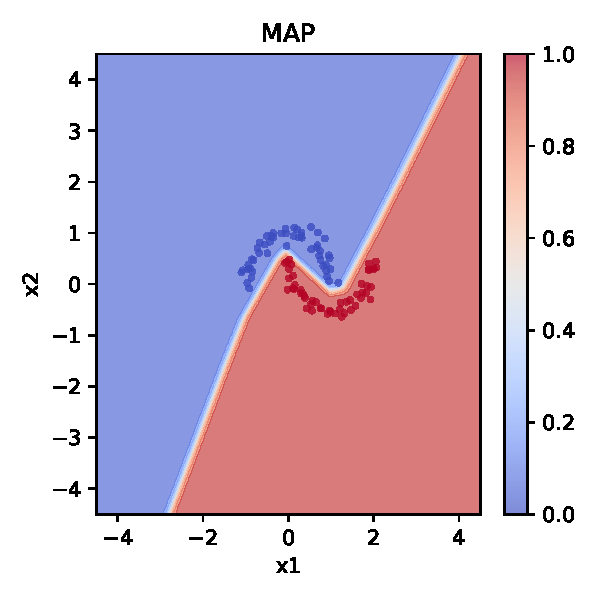
\includegraphics{images/classif_map.pdf}
  \caption{Predictions of a standard MLP. The blue and red points are training data. The color in the background represents the predicted probability $p(y \given \vec{x}, \hat{\vec{\theta}}_\text{MAP})$ at each point $\vec{x} = (x_1, x_2)^\T$ in the feature space.}
  \label{fig:classif-map}
\end{figure}

Since the network is small, we can afford computing the full Hessian matrix for Laplace approximation. In \cref{fig:classif-la}, we demonstrate the sensitivity of this method with respect to the choice of prior precision $\tau^{-2}$. For a small prior precision or large prior variance, the predictive probabilities are almost $0.5$ everywhere. The uncertainty is overestimated. As we increase the prior precision, we can recognize more meaningful structures, and the predictive distribution becomes closer to the MAP result in \cref{fig:classif-la}. A consistent pattern is that the region with predictive probabilities close to $0.5$ gets wider as we move away from the training data.

\begin{figure}[tb]
  \centering
  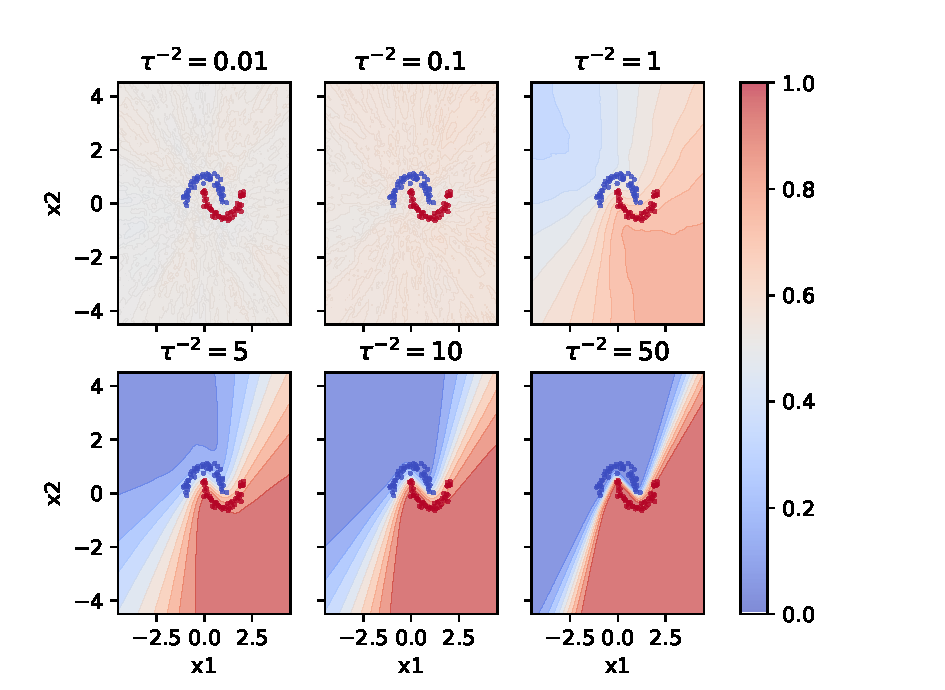
\includegraphics{images/classif_laplace.pdf}
  \caption{Laplace approximation for different prior precisions $\tau^{-2}$. Monte Carlo integration is used to approximate the predictive distribution. For each test point $(x_1, x_2)^\T$, 1000 parameters are sampled from the Gaussian approximate posterior.}
  \label{fig:classif-la}
\end{figure}

Now we construct an ensemble of 10 models with the same architecture of the MLP. The ensemble members are trained using the same hyperparameter settings, but weight initialization and batch generation are randomized. We plot five ensemble members as well as the ensemsble average in \cref{fig:classif-ensemble}. While each model is highly overconfident, some variation exists between the ensemble members. The predictive distribution given by the ensemble has a similar structure to that given by Laplace approximation with high prior precision. We observe regions of lower confidence expand towards bottom left and top right. However, the issue of overconfidence seems to persist in the other directions.

\begin{figure}[tb]
  \centering
  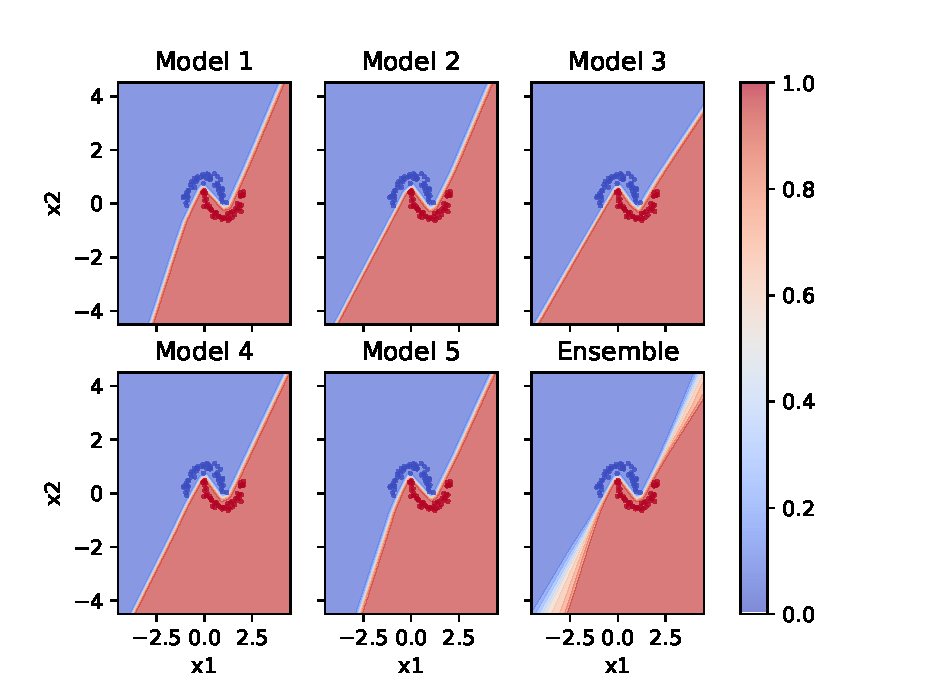
\includegraphics{images/classif_ensemble.pdf}
  \caption{Deep ensemble of 10 models. The first five plots show five individual models. The last plot shows the ensemble average.}
  \label{fig:classif-ensemble}
\end{figure}

Finally, we demonstrate Monte Carlo Dropout on the same dataset. We use the same setting to train the same MLP, but now with Dropout applied to the two hidden layers. We set the Dropout rate to $\pi = 0.2$. For such a small network, a high Dropout rate harms the prediction performance. In \cref{fig:classif-mcd}, we observe the same pattern once again: the band of low confidence extends as we move away from data, but larger regions top left and bottom right are still assigned with high confidence. We hypothesize that the unresolvable overconfidence in certain directions is a property of the network we use. \cite{kristiadiLearnableUncertaintyLaplace2021} introduced additional hidden units into the network to enhance Laplace approximation. Their approach mitigates this issue on the same dataset.

\begin{figure}[tb]
  \centering
  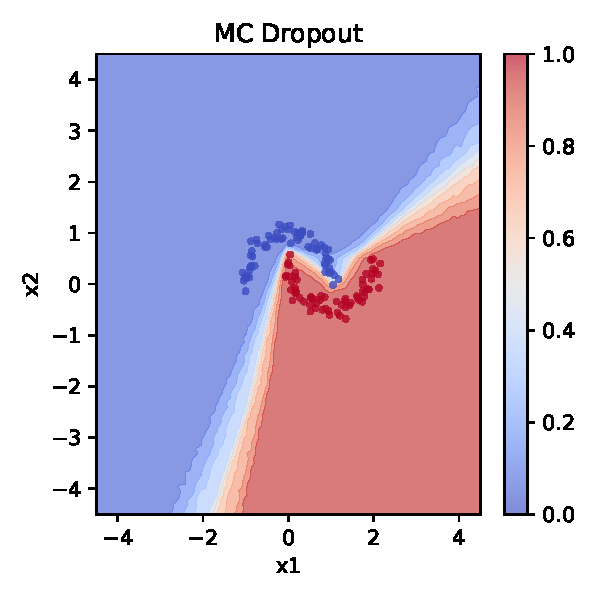
\includegraphics{images/classif_mc_dropout.pdf}
  \caption{MC Dropout. For each test point $(x_1, x_2)^\T$, a sample of 1000 parameters is used (same as for Laplace approximation).}
  \label{fig:classif-mcd}
\end{figure}

\subsection{Regression}

As a toy experiment for regression, we train an MLP with layer dimensions $[1,16,16,1]$ to learn the function $x \mapsto \sin(x)$. We generate $n = 20$ training instances as follows:
\begin{align*}
  x_i &\simiid \operatorname{Uniform}([-3, 3]), \\
  \epsilon_i &\simiid \mathcal{N}(0, 0.1^2), \\
  y_i &\defeq \sin(x) + \epsilon_i.
\end{align*}
We perform no batch generation but use standard gradient descent. The network is optimized with a learning rate of $0.1$ for 1000 epochs. The weight decay parameter is set to $10^{-6}$. \cref{fig:regr} presents the trained network (MAP estimate) and the three uncertainty quantification methods. The MAP estimate does not provide any uncertainty quantification, while we can construct error bands using the introduced methods. For Laplace Approximation, we use the last-layer variant with KFAC approximation to the Hessian and optimize the prior precision with respect to the marginal likelihood, as recommended by \cite{daxbergerLaplaceRedux2021}. The standard deviation is obtained from the Gaussian approximation to the predictive distribution. The Deep Ensemble consists of 10 models. For MC Dropout, we apply Dropout with rate $\pi = 0.2$ to both hidden layers and use the sample size 1000 for Monte Carlo integration. In the latter two approaches, we estimate the standard deviation using the empirical standard deviation over the ensemble or Monte Carlo sample.

We expect higher uncertainty when moving away from data. This is indeed observed for all three methods. Laplace Approximation is applied in a post-hoc manner. The predictive mean shown by the red curve agrees with the MAP estimate. It successfully captures the increasing uncertainty in extrapolation. Deep Ensemble exhibits higher confidence overall in comparison to Laplace approximation. \cite{lakshminarayananSimpleScalablePredictive2017b} suggests letting the model predict the error variance along with the mean, in which case overconfidence is better mitigated. The error band prodced by MC Dropout also expands when extrapolating, although not as quickly.

\begin{figure}
  \centering
  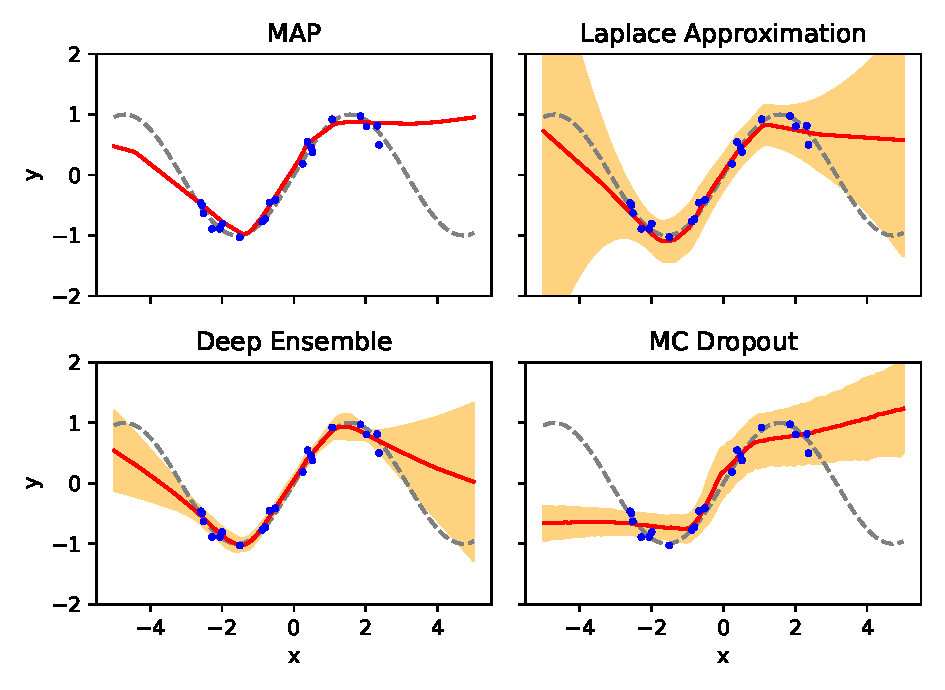
\includegraphics{images/regr_comparison.pdf}
  \caption{Comparison of MAP and uncertainty quantification methods on the regression toy dataset. The blue points as training data are sampled with Gaussian noise from the grey line. For the MAP plot, the red curve represents the prediction function. For the other plots, the predictive mean (red curve) $\pm$ two standard deviations (orange band) are shown.}
  \label{fig:regr}
\end{figure}

\newpage
\section{Discussion}

Since our illustrative examples are more of sanity checks than benchmark experiments, we compare the methods in terms of their implementation and computational cost, rather than their performance. While Lapalce approximation is applicable in a post-hoc manner, constructing the approximation is non-trivial due to challenges in Hessian computation. Furthermore, the choice of prior precision as a hyperparameter turns out to be crucial for the quality of uncertainty representation. By constrast, Deep Ensembles and MC Dropout require less implementation effort and less fine-tuning. However, they are less efficient in comparison to some variants of Laplace approximation, since it is necessary to perform multiple forward passes to obtain a single uncertainty estimate. While Deep Ensemble captures multimodality, its computational cost is much higher than the other two methods. MC Dropout seems a good alternative to Laplace approximation and Deep Ensembles if one pursues both low implementation effort and low computational cost. However, its use cases are limited to networks trained with Dropout.

\section{Conclusion and outlook}

In light of the equivalence between regulized risk minimization and MAP estimation, we presented a Bayesian view of deep learning. Our discussion was centered around the predictive distribution which accounts for both aleatroic and espistemic uncertainty as two major types of uncertainty in neural networks. We introduced three methods for approximating this predictive distribution and discussed their strengths and weaknesses.

Throughout this paper, we did not mention how to quantitatively assess these approximation methods. Benchmarking uncertainty quantification is, in fact, a difficult task, because there is no ground-truth uncertainty as reference \citep{lakshminarayananSimpleScalablePredictive2017b}. One might be able to control the aleatoric uncertainty by designing a toy experiment, but the epistemic uncertainty inside the model remains unknown. This observation also raises the question whether we can separate these two types of uncertainty. Current research shows that uncertainty disentaglement is hard \citep{mucsanyiBenchmarkingUncertaintyDisentanglement2024a,wimmerQuantifyingAleatoricEpistemic2023}. Despite the open challenges, uncertainty quantification methods have been successfully applied to active learning, medical image analysis, robotics, and earth observation \citep{gawlikowskiSurveyUQ2023}.


% \section{Introduction}
% \label{sec:intro}
% \input{chapters/introduction}
% \newpage

% \section{Conclusion}
% \label{conclusion}
% \section{Discussion}

Since our illustrative examples are more of sanity checks than benchmark experiments, we compare the methods in terms of their implementation and computational cost, rather than their performance. While Lapalce approximation is applicable in a post-hoc manner, constructing the approximation is non-trivial due to challenges in Hessian computation. Furthermore, the choice of prior precision as a hyperparameter turns out to be crucial for the quality of uncertainty representation. By constrast, Deep Ensembles and MC Dropout require less implementation effort and less fine-tuning. However, they are less efficient in comparison to some variants of Laplace approximation, since it is necessary to perform multiple forward passes to obtain a single uncertainty estimate. While Deep Ensemble captures multimodality, its computational cost is much higher than the other two methods. MC Dropout seems a good alternative to Laplace approximation and Deep Ensembles if one pursues both low implementation effort and low computational cost. However, its use cases are limited to networks trained with Dropout.

\section{Conclusion and outlook}

In light of the equivalence between regulized risk minimization and MAP estimation, we presented a Bayesian view of deep learning. Our discussion was centered around the predictive distribution which accounts for both aleatroic and espistemic uncertainty as two major types of uncertainty in neural networks. We introduced three methods for approximating this predictive distribution and discussed their strengths and weaknesses.

Throughout this paper, we did not mention how to quantitatively assess these approximation methods. Benchmarking uncertainty quantification is, in fact, a difficult task, because there is no ground-truth uncertainty as reference \citep{lakshminarayananSimpleScalablePredictive2017b}. One might be able to control the aleatoric uncertainty by designing a toy experiment, but the epistemic uncertainty inside the model remains unknown. This observation also raises the question whether we can separate these two types of uncertainty. Current research shows that uncertainty disentaglement is hard \citep{mucsanyiBenchmarkingUncertaintyDisentanglement2024a,wimmerQuantifyingAleatoricEpistemic2023}. Despite the open challenges, uncertainty quantification methods have been successfully applied to active learning, medical image analysis, robotics, and earth observation \citep{gawlikowskiSurveyUQ2023}.


\newpage

% ------------------------------------------------------------------------------
% APPENDIX ---------------------------------------------------------------------
% ------------------------------------------------------------------------------
    
\pagenumbering{Roman}

\setcounter{page}{5} % CHANGE

\appendix

% \section{Appendix}
% \label{app}
% \input{chapters/appendix}
% \newpage

\section{Electronic appendix}
\label{el_app}

Data, code and figures are provided in electronic form.

\newpage
    
% ------------------------------------------------------------------------------
% BIBLIOGRAPHY -----------------------------------------------------------------
% ------------------------------------------------------------------------------

\RaggedRight
\bibliography{bibliography}
\bibliographystyle{dcu}
\newpage

% ------------------------------------------------------------------------------
% DECLARATION OF AUTHORSHIP-----------------------------------------------------
% ------------------------------------------------------------------------------

\Large
\noindent
\textbf{Declaration of authorship} 
\vspace{0.5cm}
\noindent
\normalsize

I hereby declare that the report submitted is my own unaided work. All direct 
or indirect sources used are acknowledged as references. I am aware that the 
Thesis in digital form can be examined for the use of unauthorized aid and in 
order to determine whether the report as a whole or parts incorporated in it may 
be deemed as plagiarism. For the comparison of my work with existing sources I 
agree that it shall be entered in a database where it shall also remain after 
examination, to enable comparison with future Theses submitted. Further rights 
of reproduction and usage, however, are not granted here. This paper was not 
previously presented to another examination board and has not been published.
\\

\vspace{1cm}
\textcolor{orange}{Location, date} \\

\vspace{3cm}

\noindent\rule{0.5\textwidth}{0.4pt} \\

\textcolor{orange}{Name}

% ------------------------------------------------------------------------------

\end{document}
